\documentclass[12pt,a4paper]{scrartcl}
 \usepackage[utf8]{inputenc}
 \usepackage{amsmath}
 \usepackage{amsfonts}
 \usepackage{amssymb}
 
 \usepackage{graphicx}
 \usepackage{listings} 
 
 \usepackage[edges]{forest} 
 
 \usepackage{xcolor}
 \usepackage{hyperref}
 \usepackage{cleveref} 
 
 \hypersetup{pdftitle={main.pdf},
    colorlinks=false,
    linkbordercolor=red
 } 
\definecolor{folderbg}{RGB}{124,166,198}
\definecolor{folderborder}{RGB}{110,144,169}
\newlength\Size
\setlength\Size{4pt}
\tikzset{%
  folder/.pic={%
    \filldraw [draw=folderborder, top color=folderbg!50, bottom color=folderbg] (-1.05*\Size,0.2\Size+5pt) rectangle ++(.75*\Size,-0.2\Size-5pt);
    \filldraw [draw=folderborder, top color=folderbg!50, bottom color=folderbg] (-1.15*\Size,-\Size) rectangle (1.15*\Size,\Size);
  },
  file/.pic={%
    \filldraw [draw=folderborder, top color=folderbg!5, bottom color=folderbg!10] (-\Size,.4*\Size+5pt) coordinate (a) |- (\Size,-1.2*\Size) coordinate (b) -- ++(0,1.6*\Size) coordinate (c) -- ++(-5pt,5pt) coordinate (d) -- cycle (d) |- (c) ;
  },
}
\forestset{%
  declare autowrapped toks={pic me}{},
  pic dir tree/.style={%
    for tree={%
      folder,
      font=\ttfamily,
      grow'=0,
    },
    before typesetting nodes={%
      for tree={%
        edge label+/.option={pic me},
      },
    },
  },
  pic me set/.code n args=2{%
    \forestset{%
      #1/.style={%
        inner xsep=2\Size,
        pic me={pic {#2}},
      }
    }
  },
  pic me set={directory}{folder},
  pic me set={file}{file},
}
 
 \title{\textbf{Prototype of a pipeline for reproducible nuclear data evaluation} \\[2ex] User manual}
 \date{March 24, 2021\\v0.1.0}
 \author{Georg Schnabel \\ \href{mailto:georg.schnabel@nucleardata.com}{georg.schnabel@nucleardata.com}}
 
 \begin{document}

 \maketitle
 \begin{abstract}
This document provides instructions to set up a pipeline for nuclear data evaluation using the nuclear models code TALYS.
Relying on the Docker technology for virtualization, the pipeline is easy to install.
The pipeline performs a fully automated and reproducible evaluation of neutron-induced cross sections of Fe-56.
The pipeline can be explored and modified either using a terminal and the typical Linux command line tools or a graphical user interface accessible via a web browser.
The evaluation features automatic uncertainty correction of experimental data and tuning the model parameters using the Levenberg-Marquardt algorithm.
The mathematical details of the evaluation are outside the scope of this document whose focus is on the technical aspects to get the pipeline running.
The proper working of the pipeline can be tested on a desktop computer.
For a full scale evaluation, either a multicore machine or a cluster with SSH access is strongly recommended.
The manual explains the setup of the pipeline on Linux.
It may be possible to set up the pipeline on a Windows machine but we have not tested that.
 \end{abstract} 
 \newpage
 \tableofcontents
 \newpage 

 \section{Introductory remarks}
 The ability to reproduce complex scientific workflows becomes more and more an important concern.
 Increasing awareness that many past studies are impossible to reproduce has now even led to the term \textit{reproducibility crisis}.
 The situation in nuclear data evaluation is not different.
 Many choices related to the selection of the experiments, corrections applied to the experimental data, and the choice of evaluation method are often not well documented enough to enable the reproduction of an evaluation.
 This circumstance hinders progress and building on the efforts from the past.
 
 Motivated by these observations, this document presents an example of a reproducible and automated pipeline for nuclear data evaluation.
 The evaluation algorithms used as well as the selection and correction of experimental data are automated as a well-structured sequence of scripts.
 This sequence of scripts is referred to as \textit{pipeline}.
 Anyone interested in the details of the evaluation can find them in the pipeline whose usage is explained in this document.
 It is also my hope that the pipeline will be a helpful example in the ongoing discussion about the best way to make evaluations reproducible and how to incorporate expert knowledge into automated evaluation procedures.
 
 The pipeline has been created for an evaluation of neutron-induced cross sections of Fe-56.
 In principle, it can be modified to produce evaluations of other isotopes, to use a different set of experimental data, or optimize other model parameters than in the default configuration.
 This document will provide explanations and pointers to effect such modifications.
 However, in view of the complexity and the tremendous number of different choices possible in an evaluation, covering all potential use cases is clearly out of reach in this document.
 As the pipeline is written in R, a working knowledge of the programming language R and the willingness to develop some familiarity with the pipeline is required to effect modifications not discussed in this document.
 
 \section{Brief description of how the evaluation pipeline works}
 The pipeline is a collection of scripts to perform a model-based evaluation of an isotope using the TALYS code.
 The scripts in the pipeline are written in the programming language R.
 They have to be called in the correct order because the required input for each script is the output of previous scripts.
 There is a master script that executes all the scripts in the pipeline in the correct order.
 The input to the pipeline is a TALYS input file and an additional configuration file.
 The TALYS input file determines which isotope should be evaluated and the specific values for the TALYS parameters to be used.
 The configuration file contains the setup of the pipeline, such as the energy grid that should be used for the TALYS calculations or the number of iterations in the Levenberg-Marquardt optimization algorithm.
 The output of the pipeline is a collection of \textit{tar} files, each of them containing all result files produced by a TALYS calculation with a specific choice of model parameters.
 These \textit{tar} files can be provided as input to TASMAN and TEFAL written by Arjan Koning to produce an ENDF file.
 
\section{Bundling the pipeline - the Docker image} 
The scripts in the pipeline rely on many different components, such as a MongoDb database, the R programming language, and several custom R packages, some of which require functionality only available under Linux.
The installation and setup of all the individual components is quite tedious.
Therefore a Dockerfile was created that performs all the required installation steps automatically and produces a Docker image. This Docker image serves as the blue-print to instantiate Docker containers. A Docker container can be regarded as a light-weight virtual machine that runs Linux on top of the base operating system which can be either Linux, Windows, or MacOS.
In addition to facilitating the setup, the Docker mechanism completely separates and decouples the pipeline from the underlying operating  system.
In other words, we do not mess around in any way with the configuration of your operating system.

The official Docker website is located at \url{https://www.docker.com}.
Please consult the information on this website for more information about Docker.
In particular, the installation of Docker Community Edition (CE), which is free of charge, is detailed at \url{https://docs.docker.com/get-docker/}.
The Docker application is an essential requirement to perform the installation of the evaluation pipeline as described in this document.
Whether Docker is installed on your system can be checked by running in a terminal
\begin{verbatim}
  docker version
\end{verbatim}
If Docker is installed, you should see information about the installed Docker version and you can proceed to the next section.

 \section{Installation of the evaluation pipeline}
We mean by \textit{installation of the pipeline} the installation of the Docker image, the creation of a Docker container based on the Docker image, and the necessary configuration \textit{within} the container, and potentially some actions that need to be performed \textit{outside} the container.

There are two possible setups.
The container can be set up so that the complete pipeline including running TALYS is performed \textit{within} the container. This mode of operation is recommended for testing and to get familiar with the pipeline. We will discuss it first in~\cref{subsec:install_basic}.
Afterwards, building on the successful basic setup, we explain in~\cref{subsec:install_multicore} the necessary setup steps on a cluster or multicore machine and the configuration within the container to enable parallel computing.
In the latter mode of operation, the machine running the Docker container needs to be able to access the multicore machine via SSH.
It is also possible to run the Docker container itself on the multicore machine.

 \subsection{Basic installation}
 \label{subsec:install_basic}
  
 First, download and unpack the file at
 \\[2ex]
 \indent\url{https://github.com/gschnabel/eval-fe56-docker/archive/master.zip}
 \\[2ex]
 \noindent 
 Unpacking creates a new folder \path{eval-fe56-docker-master}.
 Open the file \path{install_all.sh} present in this folder in a text editor. At the beginning of this file are the two lines
\begin{verbatim}
  username="username"
  password="password"
\end{verbatim}
 These credentials will be used for the creation of a user account within the Docker image.
 Furthermore, they will be required to access the pipeline via a web browser.
 The command line instructions in the manual assume these credentials. 
However, you can change the username and the password between the quotation marks to your liking.
 
 Depending on your internet speed, the following instruction may take up to an hour.
 Open a terminal and change into the folder \path{eval-fe56-docker-master}.
 Make sure that this folder, now the current working directory, contains the file \path{Dockerfile}.
Then in the terminal run
\begin{verbatim}
  docker build -t eval-fe56-img:latest . 
\end{verbatim}
 Please note that the final point is part of the command.
 This instruction creates a so-called \textit{Docker image} by downloading all required components (e.g., MongoDb, TALYS, R, etc.) from various resources on the net and assembling them as a Docker image.
 If everything went well, the pipeline is now successfully installed on your computer.
 If you wish, you can delete the folder \path{eval-fe56-docker-master} now because it was only needed for the creation of the Docker image.

 \subsection{Testing the basic installation}
 \label{subsec:test_basic_install}
 As a first verification step, we test whether the Docker image has been successfully created.
 To that end, open a terminal window and run the command
\begin{verbatim}
  docker images
\end{verbatim}
 It will display a listing of available Docker images.
 If a row is present with \textit{eval-fe56-img} as the repository name, the creation of the Docker image was successful.
 
 Now let us create a container based on the Docker image.
 In a terminal window run the command
\begin{verbatim}
  docker run -it -p 9090:8787 --name eval-fe56-cont \
             eval-fe56-img:latest interactive
\end{verbatim}
 After a few seconds, you will see a command prompt starting with \verb#username@# followed by a long hexadecimal string.
 You are in a Linux session \textit{inside} the container.
 
 To test the full pipeline, we need to run it.
 When typing the following instructions, whenever the word \verb#username# appears, you need to replace it by the username chosen for the creation of the Docker image.
 Change to the directory containing the pipeline
\begin{verbatim}
  cd /home/username/eval-fe56
\end{verbatim}
  The directory structure inside the pipeline and more general inside the container will be discussed in a later section.
  Run the pipeline by typing
\begin{verbatim}
  Rscript --vanilla run_pipeline.R
\end{verbatim}
It usually takes between five to ten minutes until the command completes.
During execution various messages will appear in the terminal.
Pay attention to the messages enclosed by a sequence of \# characters informing about the start or the termination of a step.
The pipeline consists of nine steps in total.

If the last step finished successfully, you will be back at the command prompt.
Change to the directory containing the TALYS results
\begin{verbatim}
  cd /home/username/talysResults
\end{verbatim}
Display the content of this directory by typing
\begin{verbatim}
  ls
\end{verbatim}
If you see a list of \textit{tar} archives, the full pipeline executed successfully. Congratulations!
Finally, you can get a first glimpse at the graphical user interface.
Open the web browser of your choice and go to the address
\begin{verbatim}
  http://localhost:9090
\end{verbatim}
When you see the page prompting you for a username and a password,
use the credentials you specified during the creation of the Docker image.
After the successful login, you will see an integrated development environment (IDE) to write R code.
At this moment, you can close your web browser or the tab showing the web page.
If you got curious about this IDE, which is called \textit{Rstudio}, you can learn more at \url{https://resources.rstudio.com/}.
Noteworthy, the pipeline could also have been started from the IDE accessible via the web browser.

To shut down the container, either execute inside the container the command
\begin{verbatim}
  exit
\end{verbatim}
or in a terminal \textit{outside} the container, run the command
\begin{verbatim}
  docker stop eval-fe56-cont
\end{verbatim}
If at a later point in time, you want to start the container again, run the command
\begin{verbatim}
  docker start eval-fe56-cont
  docker attach eval-fe56-cont
\end{verbatim}
The second command is only necessary if you want to work with a shell prompt \textit{inside} the container.
It is however not needed to manage the pipeline via the graphical user interface accessible via a web browser.

If you want to dispose of the container, all data produced by the run of the pipeline are then discarded,
run the command
\begin{verbatim}
  docker stop eval-fe56-cont
  docker rm eval-fe56-cont
\end{verbatim}

\subsection{Running the pipeline on a multicore machine}

The full evaluation of Fe56 requires a multicore machine or cluster.
We first explain the use of a multicore machine because the setup is easier.
The ballpark of the runtime on a machine with about 80 cores is about twelve hours.
The runtime depends linearly on the number of cores.

First, create the following directory structure on your file system,
which will be filled with the data generated during the run of the pipeline:
\begin{verbatim}
  mkdir eval-fe56
  cd eval-fe56
  mkdir outdata
  mkdir talysResults
\end{verbatim}

Let \verb#<PATH># be the absolute path of the \verb#eval-fe56# folder.
If you are on a Linux machine, figure out your user id \verb#UID# and group id \verb#GID#,
e.g., by using the command
\begin{verbatim}
  cat /etc/passwd | grep <your username>
\end{verbatim}
The first number of the output is the \verb#UID# and the second number the \verb#GID#. 
There are four modes to run the pipeline:
\begin{itemize}
  \item \emph{interactive} - create a container and immediately log in as the default user
  \item \emph{interactive\_root} - create a container and immediately log in as the root user
  \item \emph{test\_eval} - create a container and perform a test evaluation (non-interactive mode)
  \item \emph{full\_eval} - create a container and perform a full evaluation (non-interactive mode)
\end{itemize}
The template of the command to start the container with the pipeline is given by
\begin{verbatim}
docker run -it -p 9090:8787 \
           -v <PATH>/outdata:/home/username/eval-fe56/outdata \
           -v <PATH>/talysResults:/home/username/talysResults \
           -v /dev/shm:/dev/shm \
           -e extUID=<UID> -e extGID=<GID> -e maxNumCPU=32 \
           --name eval-fe56-cont eval-fe56-img \
           <mode> 
\end{verbatim}
The backslash at the end of a line indicates that the next line still belongs
to the current instruction.
Under Linux, the folder \verb#/dev/shm# is mapped into main memory.

You may want to use mode \emph{test\_eval} first to see whether the command
works correctly.
At the end of that run you should have some tar archives in the folder
\verb#talysResults# and a bunch of folders numbered from \verb#01# to
\verb#09#.
After you have seen that everything works, you can delete the files and folders
in \verb#outdata# and \verb#talysResults# and run a full evaluation by using
the mode \emph{full\_eval}.
Using 32 cores (\verb#maxNumCPU=32#) leads to a storage need of about 3 GB in
\verb#/dev/shm# and 23 GB of main memory. For reference, using 32 cores the
pipeline finished in about 16 hours on a multicore machine.

If something goes wrong, you can force the stopping of the container by
running
\begin{verbatim}
  stop eval-fe56-cont
\end{verbatim}


 \subsection{Connecting the pipeline to a cluster}
 \label{subsec:install_multicore}
 We assume that you have successfully performed the installation of the pipeline as described in~\cref{subsec:install_basic}.
 In the default configuration of the pipeline, all computations are performed \textit{inside} the Docker container.
 For full scale evaluations, it is strongly recommended to run the pipeline in combination with a multicore machine or cluster.
 For the time being, Linux must be installed on the multicore machine or cluster.

 In the previous section we briefly showed how the pipeline can be run inside the Docker container on a multicore machine.
 The pipeline container can also run on a computer which connects to the multicore machine via SSH to perform the
 required calculations there.
 This configuration is depicted in the following graph.
 \begin{center}
 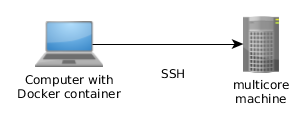
\includegraphics[scale=0.6]{graphs/multicore_config.png}
 \end{center}
 Please note that it is perfectly fine to run the Docker container also on the multicore machine.
 
 Concerning the use in combination with a cluster, we assume that the cluster is a collection of processing units (can be thought as individual computers) which have access to a common filesystem.
 At least one processing unit needs to be accessible via SSH from the computer running the Docker container.
 In addition, it must be possible to execute instructions on all the processing units (e.g., also via SSH). 
 This mode of operation of the pipeline is depicted in the following graph.
 \begin{center}
 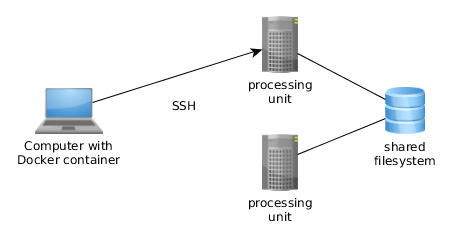
\includegraphics[scale=0.6]{graphs/cluster_config.png}
 \end{center}
 It is perfectly fine to run the Docker container on one of the processing units.
 
 The setup of the pipeline in combination with a multicore machine is almost identical to the one with a cluster.
 The setup with a multicore machine can be regarded as a special case of a cluster with only one processing unit.
 The following instructions have therefore to be repeated for each processing unit.
 We will therefore from now on only use the term \textit{processing unit}.
 The necessary steps on a processing unit (except step 4) are:
 \begin{enumerate}
  \item Installation of the interpreter for the programming language R
  \item Installation of required R packages
  \item Creation of necessary folders on the shared filesystem
  \item (Configuration in the Docker container)
  \item Launch of the script watching for new calculation requests 
 \end{enumerate}
 \textit{Within} the Docker container, a few configuration variables concerning the SSH connection must be changed, which is step 4.
 In step 4 also the watch script is transferred to the shared filesystem, which is then launched in step 5.

 Following, we will go through each of the steps in more detail.
 For the installation of the R interpreter, admin privileges are strongly recommended.
 Furthermore, in the scenario with a cluster, the same user should exist on each of the processing units to avoid problems with read and write permissions on the shared filesystem.
 
\subsubsection{Installation of the R interpreter}

Log in to the processing unit via SSH.
You can check whether R is installed and the available version by executing the command
\begin{verbatim}
  R -e 'R.version.string'
\end{verbatim}
If the command executes successfully and the version is greater or equal 3.5, an appropriate version of R is already installed and you can proceed to the next section.
Otherwise, if you have root privileges and use \textit{Ubuntu} as Linux distribution, you can follow the installation instructions at \url{https://www.digitalocean.com/community/tutorials/how-to-install-r-on-ubuntu-18-04}.
Tutorials for other operating systems can also be found on the web.
The authoritative reference for the R programming language is \url{https://www.r-project.org/}.

If you don't have admin privileges on the processing unit, ask your system administrator to do the installation for you.
In principle, it is possible but more involved and error prone to install without admin privileges.
Information concerning this type of setup can also be found on the official website mentioned above.


\subsubsection{Installation of required R packages}

Log in to the processing unit via SSH.
Make sure to log in under the user account that will be used for executing  TALYS calculations.
To install the required R packages, execute
\begin{verbatim}
  Rscript -e 'install.packages("digest", repos="https://cran.rstudio.com")'
  Rscript -e 'install.packages("data.table", repos="https://cran.rstudio.com")'
\end{verbatim}
Afterwards, we need to install a custom package for handling the preparation and reading the results of TALYS calculations.
First, download the package and unzip it, e.g., by using the commands
\begin{verbatim}
  wget https://github.com/gschnabel/TALYSeval/archive/master.zip
  unzip master.zip
\end{verbatim}
The result of these instructions is a new directory named \path{TALYSeval-master}.
As an aside, navigating in a browser to \verb#https://github.com/gschnabel/TALYSeval# will show the structure of the package and more details about it.
Now we can install the R package by running the command
\begin{verbatim}
  R CMD INSTALL TALYSeval-master
\end{verbatim}
At this stage, all required R packages are installed on the processing unit.
You can test whether the installation was successful by starting the \textit{R interpreter} by running the command
\begin{verbatim}
  R
\end{verbatim}
Once you are at the prompt of the R interpreter, run the following commands
\begin{verbatim}
  library(digest)
  library(data.table)
  library(TALYSeval)
\end{verbatim}
If the installation of a package failed, you will see an error message.
Finally, quit the R interpreter by typing
\begin{verbatim}
  q()
\end{verbatim}
As a reminder, the installation instructions of this section have to be repeated on every processing unit that should participate in the execution of TALYS calculations.

 \subsubsection{Creation of necessary folders on the shared filesystem}
 \label{subsubsec:create_shared_folder}
 On the filesystem accessible from all the processing units, two folders need to be created.
 Both of them need to be read- and writeable by the user account under which the TALYS calculations will be executed.
 Assuming that your user account is named \verb#username#, you can use the following locations:
\begin{verbatim}
  mkdir /home/username/remcalcdir
  mkdir /home/username/TALYSresults
\end{verbatim}
The first folder \path{remcalcdir} is used for communication between the Docker container accommodating the evaluation pipeline and the cluster/multicore machine.
The second folder \path{TALYSresults} will store a collection of \textit{tar} files containing TALYS calculation results which are the final output of the pipeline.
 
 \subsubsection{Configuration in the Docker container}
 \label{subsubsec:install_remote_config_container}
 
 If you are not sure whether the container has launched, check by running in a terminal the command
\begin{verbatim}
  docker ps -a
\end{verbatim}
You will see a list of all available containers and their execution state under the \verb#STATUS# column.
If the container \verb#eval-fe56-cont# has exited, you need to start it up again by running
\begin{verbatim}
  docker start eval-fe56-cont
\end{verbatim}
It would be a possibility to configure the container from a bash shell inside the container.
As a reminder, running the command \verb#docker attach eval-fe56-cont# would get you to such a shell.
For convenience, we are going to use the graphical user interface accessible via a web browser instead.
Open your favorite web browser and go to the address
\begin{verbatim}
  http://localhost:9090
\end{verbatim}
When prompted for a password and a username, use the credentials provided during the creation of the Docker image in~\cref{subsec:install_basic}.
After the successful login, you see a graphical user interface with several panes.
The pane at the bottom right provides a view of the filesystem \textit{inside} the container.
By default, the folders you see are located in the user home directory.
Now perform the following actions:
\begin{enumerate}
  \item Click on the folder \path{eval-fe56} in the folder view to enter this folder.
  \item Click on the file \path{config.R} in the folder view to open this file.
\end{enumerate}
After these two steps, the content of the file \path{config.R} should appear on the left in your browser window.
In the programming language R, assigning a value to a variable is done using the operator \verb#<-#.
Knowing this, you see that the majority of code in this file are assignments of strings and values to variables.
The purpose of these configuration variables is to set up the behavior and specifics of the pipeline.
Now we will make the necessary changes so that the pipeline can launch computations on your multicore machine or cluster.

Locate the block of variables
\begin{verbatim}
  ssh_login <- "..."
  ssh_pw <- "..."
\end{verbatim}
Please note that in your case the dots between the quotation marks will be something else.
Replace the strings between the quotation marks by your credentials to log in to the multicore machine or cluster.
For instance, if you logged in to your cluster at \verb#cluster.com# with user name \verb#user# and password \verb#pw#, you would end up with
\begin{verbatim}
  ssh_login <- "user@cluster.com"
  ssh_pw <- "pw"
\end{verbatim}
If you don't like to have the password in clear text in this file, an alternative option is to configure the SSH connection for password-less login.
In this case, you would be required to use the bash prompt inside the container (accessible by typing \verb#docker attach eval-fe56-cont#).
Furthermore, some configuration would then be necessary on the cluster.
Instructions about this type of setup can be found at numerous places on the net, e.g., here
\begin{verbatim}
  https://linuxize.com/post/how-to-setup-passwordless-ssh-login/
\end{verbatim}
So far we have told the pipeline how to connect via SSH to the cluster.
The mechanism to launch TALYS calculations is to use the filesystem on the cluster for communication and data exchange.
Specifically, the pipeline creates files representing calculation requests in a specified folder, which is periodically scanned by a watch script running on the processing units.
If such a watch script spots a file with a calculation request, it will launch the respective calculation.
We have already created this data exchange folder in~\cref{subsubsec:create_shared_folder}.
If you have adopted the suggestion there, it is located at~\path{/home/username/remcalcdir} with \path{username} being replaced by your actual username on the cluster.
To tell the pipeline where this folder is located on the cluster, modify the variable \verb#calcdir_rem# accordingly in the configuration file.
The relevant line may then look like this:
\begin{verbatim}
  calcdir_rem <- "/home/username/remcalcdir"
\end{verbatim}
As a final required modification, we need to specify the folder on the shared filesystem on the cluster where the final TALYS results are stored.
This information is defined in the variable \verb#savePathTalys#.
If you adopted the suggestion on the folder name of~\cref{subsubsec:create_shared_folder}, you should modify the line containing the assignment to \verb#savePathTalys# to have the following:
\begin{verbatim}
  savePathTalys <- "/home/username/TALYSresults"
\end{verbatim}
The string \verb#username# needs to be changed to your actual username on the cluster.

Next we specify the path to the TALYS executable on the remote machine and in which folder TALYS calculations should be run on the remote machine.
Both settings can be found in the line
\begin{verbatim}
  talysHnd <- initClusterTALYS( ... )  
\end{verbatim}
In the arguments of the function \verb|initClusterTALYS|, you will find the mention of \verb|talysExe = "..."|.
Replace whatever you find between the quotation marks by the path to the TALYS executable on the shared filesystem of the remote machine.
Further, there is a part \verb|TMPDIR = "..."|. 
Replace whatever you find between the quotation marks by the path on the remote machine where the TALYS calculations are to be performed.
Due to the large number of files produced by TALYS, it is recommended to choose a path that resides on a RAM drive.
Under many Linux distributions, everything under \path{/dev/shm} resides in main memory.
So the path \path{/dev/shm/talysTemp} may be a good choice.

Now scroll to the beginning of the file and set
\begin{verbatim}
  containerTest <- FALSE
\end{verbatim}
Setting this variable to \verb|FALSE| tells the pipeline to not start TALYS inside the container.
Launching TALYS is the responsibility of the remote machine.

Even though many more options can be tweaked in the \verb|config.R| file, at this point all necessary modifications \textit{inside} the container are implemented to run the pipeline in combination with a remote machine or cluster.
To check that everything works as expected, click on the \verb|Source| button located near the top-right corner of the editor pane which shows the file content.
This will save the modifications permanently to \verb|config.R| and execute the configuration.

If everything goes well, no error message will appear.
If an error message appears, double check the modifications you have made.
Maybe you have deleted by coincidence a required quotation mark around a string.
By clicking on \verb|Edit| in the menu at the top, and then \verb|Back| you can undo your changes until you locate the problematic line.

The last required action in this step is to transfer the script that monitors calculation requests and launches calculations to the remote machine.
After having pushed the \verb|Source| button, you see an additional pane in the bottom left of your browser with at least two tabs.
The active tab is named \verb|Console|.
This console allows to type R instructions and execute them by pressing \verb|Enter|.
To transfer the watch script, type in this console
\begin{verbatim}
  slaveSetupCmd(nohup = FALSE, launch = FALSE)
\end{verbatim}
and press \verb|Enter|.
This command will produce a few lines of output in the console.
If everything goes well, the output should look something like this:
\begin{verbatim}
  ssh - connecting to remote machine...
  ssh - ...connection established
  Prepare files on local and remote machine...
  Shared connection to localhost closed.
  Rscript --vanilla .../jobControl/nodeController.R
\end{verbatim}
Pay attention to the presence of the line with \verb|connection established| indicating the successful connection to the remote machine via SSH.
The last output line starting with \verb|Rscript| shows the path on the remote machine to the watch script.
The three dots will be something different in your case.
The complete command \verb|Rscript --vanilla ...| is supposed to be run on the cluster in the next step.
Copy it to the clipboard or write it down.
You will need it later.

\subsubsection{Launch of the watch script}
\label{subsubsec:launch_watchscript}

The watch script in the file \path{nodeController.R} needs to be launched on each processing unit that is supposed to participate in the calculations.
Even if you have several processing units with access to a shared filesystem, we recommend to try the pipeline with only one participating processing unit first.
After a successful test of the full pipeline in the next section, you can come back to this section and launch the watch script on the other processing units as well.
This approach facilitates stopping a bunch of TALYS calculations if something goes wrong.

Let's start.
Log in via SSH to the processing unit that should run the calculations.
Now you have two options.
You can execute the command (with \verb|...| replaced by the path you obtained at the end of the last section):
\begin{verbatim}
  Rscript --vanilla .../jobControl/nodeController.R
\end{verbatim}
This will start the watch script in the foreground.
The advantage is that error messages (if any) are printed in your terminal which facilitates debugging.
Furthermore, you can easily stop the execution of the watch script by pressing \verb|CTRL+C| if needed.

Alternatively, you can launch the watch script in the background:
\begin{verbatim}
  nohup Rscript --vanilla .../jobControl/nodeController.R &
\end{verbatim}
This option is to be preferred if you want to launch the watch script on several processing units.
The watch scripts stays active even if you disconnect from the remote machine.
If you want to check whether the watch script is really running in the background, run
\begin{verbatim}
  ps aux | grep "nodeController"
\end{verbatim}
The output of this command should contain a line associated with the command above.
Pay attention that the line does not contain the string \verb#grep# but does contain the string \verb#Rscript ... nodeController.R#.

It is important to know how to stop the watch script.
The case where it runs in the foreground has been discussed above.
For the case where it runs in the background, a way to stop the watch scripts on all processing units at once is to delete all files whose name starts with \verb|active_| in the \path{jobControl} directory, i.e.,
\begin{verbatim}
  rm .../jobControl/active_*
\end{verbatim}
It may take up to a minute until all watch scripts are shut down.

Alternatively, you can locate the process ID of the scripts by, e.g., 
\begin{verbatim}
  ps aux | grep "nodeController.R"
\end{verbatim}
and kill them.
Retrieving the process id and killing the scripts can be done in one step with the command
\begin{verbatim}
  ps aux | grep 'nodeController' | awk '{print $2}' | xargs kill
\end{verbatim}
Importantly, in this way you only stop the watch scripts on the current processing unit.
In addition, if stopping the watch script that way, the next time you try to start it up, it will complain about an existing file whose name starts with \verb|active_|.
After you have deleted the reported file, starting up the watch script should work again.

 \subsection{Testing the pipeline in combination with a cluster or multicore machine}
 \label{subsec:test_pipeline_cluster}

We assume that you have set up the Docker container and remote machine to work together as explained in~\cref{subsec:install_multicore}.
In particular, this means that the configuration inside the Docker container has been done according to \cref{subsubsec:install_remote_config_container} and the watch script is running on the remote machine as explained in~\cref{subsubsec:launch_watchscript}.

Log in to the machine where the Docker container resides.
Open a terminal window and type
\begin{verbatim}
  docker ps -a
\end{verbatim}
There should be a line associated with the container \verb|eval-fe56-cont|.
If the container is not running yet (i.e., has status exited), start it up by typing
\begin{verbatim}
  docker start eval-fe56-cont
\end{verbatim}
Once the container is started, you can get access to a shell inside the container by executing
\begin{verbatim}
  docker attach eval-fe56-cont
\end{verbatim}
As a result of this command, you will see a prompt beginning with \verb|root@|.
This prompt indicates that we are inside the container, which is decoupled from your base operating system.
Switch from the root user to the user created during the installation.
You have defined the user credentials at the start of~\cref{subsec:install_basic}.
If you don't want to scroll back, you can figure out the username by  running
\begin{verbatim}
  cd /home; ls
\end{verbatim}
to print the username, which is the name of the directory listed.
Switch from the root user to this user by executing (with \verb|username| replaced by the actual username)
\begin{verbatim}
  su username
\end{verbatim}
 Change to the directory containing the pipeline
\begin{verbatim}
  cd /home/username/eval-fe56
\end{verbatim}
  The directory structure inside the pipeline and more general inside the container will be discussed in a later section.
  Run the pipeline by typing
\begin{verbatim}
  Rscript --vanilla run_pipeline.R | tee pipeline.log
\end{verbatim}
It usually takes between five to ten minutes until the command completes.
During execution various messages will appear in the terminal.
Pay attention to the messages enclosed by a sequence of \# characters informing about the start or the termination of a step.
The pipeline consists of nine steps in total.

You can also log in to the processing unit that is supposed to perform the calculation and run, e.g.,
\begin{verbatim}
  top
\end{verbatim}
to monitor activity.
Specifically, pay attention to whether TALYS calculations are launched or not.

If the last step has finished successfully, you will be back at the command prompt.
Change to the directory containing the TALYS results
\begin{verbatim}
  cd /home/username/talysResults
\end{verbatim}
Display the content of this directory by typing
\begin{verbatim}
  ls
\end{verbatim}
If you see a list of \textit{tar} archives, the full pipeline executed successfully.
If some error occurred, the content of the file \verb|pipeline.log| may give some clue about the problem.
You can contact the creator of this pipeline\footnote{The email address can be found on the first page of this manual.} for guidance how to solve it.

 \section{Exploring the content of the Docker container}
 
 It is an advantage during installation that the Docker image and the therefrom created container can be treated as black boxes.
 In order to make changes to the pipeline, however, it is helpful to understand the internal structure of the Docker container, and in particular the structure of the evaluation pipeline.
 In this section, we first elaborate on the basic folder structure, then zoom onto the folder containing the pipeline, and finally discuss the R packages used by the scripts in the pipeline.

\subsection{Basic folder structure}
Since Linux is running in the container, the typical folder structure for that operating system is present.
In particular, the path \path{/home} contains the home directories of the users.
Only one (non-root) user is created during the Docker setup and therefore only one folder is present under the \path{/home} folder.
The name of this subfolder is identical to the username created during the Docker setup in~\cref{subsec:install_basic}.
For the following let us assume that the username is \verb|username|.
The folder \verb|/home/username| contains all the folders related to the pipeline.
The following tree listing shows the most important folders:

\begin{forest}
  pic dir tree,
  where level=0{}{% folder icons by default; override using file for file icons
    directory,
  },
[/home/username
  [install]
  [calcdir]
  [remcalcdir]
  [eval-fe56]
  [talys]
  [talysResults]
]
\end{forest}

The role of these folders during installation and then during the execution of the evaluation pipeline is briefly outlined in the following:
\begin{description}
\item[install]
This folder contains files that have been downloaded and used during installation.
Noteworthy, the subfolder \path{Rpackages} contains the code of the R packages used by the scripts in the pipeline.
Examples of functionality provided by these packages are access to the EXFOR library and communication with a cluster via SSH.
\item[calcdir]
This folder is used by the R package \verb|remoteFunctionSSH| which provides functionality to execute R code on a remote machine.
The package \verb|clusterSSH| makes use of \verb|remoteFunctionSSH| and provides additional functionality related to launching calculations in parallel.
Also this latter package adds files and folders in \path{calcdir}.
Noteworthy, the folder \verb|calcdir/functions| contains folders and files associated with functions registered for remote execution.
\item[remcalcdir]
The content of the folder \verb|remcalcdir| mirrors that of the folder \verb|calcdir|.
Using two synchronized folders, one in the container and one on the remote machine, is the mechanism employed by package \verb|remoteFunctionSSH| to transfer functions to the remote machine for execution.
In the basic configuration as described in~\cref{subsec:install_basic}, the remote machine is the Docker container itself, which explains why \path{calcdir} and \path{remcalcdir} reside at the same location.
However, in the configuration with a cluster as described in~\cref{subsec:install_multicore}, a folder on the remote machine specified by the user is used instead of the folder \path{remcalcdir} in the container.  

\item[eval-fe56]
This folder contains the scripts of the evaluation pipeline.
The file \path{eval-fe56/config.R} contains variables to configure the pipeline, such as the SSH credentials to connect to the remote machine.
The folder \path{eval-fe56/script} contains a sequence of scripts ordered by a number given as prefix in their filenames.
The script \path{eval-fe56/run_pipeline.R} executes all scripts in the pipeline in the correct order.
More details about the scripts in the pipeline will be given in~\cref{subsec:structure_pipeline}.

\item[talys]
This folder contains the source files of the nuclear models code TALYS\footnote{www.talys.eu}, data libraries, the TALYS documentation, and the executable.
This folder will only be created if the installation of TALYS has been selected as an option for the installation.
By default, it is installed.

\item[talysResults]
The result of the pipeline are a number of TALYS calculations with varied model parameters.
The result files of each calculation are stored as a compressed \textit{tar} archive in this folder.
These files may be either passed one by one to the TEFAL code\footnote{The TEFAL and TASMAN code written by Arjan Koning are part of the T6 code system which is employed to produce the TENDL library.} to produce random files in the ENDF format or to a modified version of TASMAN to produce one ENDF file with covariance information.

\end{description}
 
 \subsection{Structure of the evaluation pipeline}
 \label{subsec:structure_pipeline}

 The evaluation pipeline is located in the folder \path{eval-fe56} in the user home directory inside the Docker container.
 Here is an expanded tree of the directory structure with important files and directories:

\begin{forest}
  pic dir tree,
  where level=0{}{% folder icons by default; override using file for file icons
    directory,
  },
  [eval-fe56
    [config.R,file]
    [run\_pipeline.R,file]
    [script
      [01\_prepare\_experimental\_data.R, file]
      [..., file]
      [utils]
    ]
    [indata
    ]
    [outdata
    ]
  ]
\end{forest}
 
 In the following we briefly discuss each of the files and directories in turn:
\begin{description}
\item[config.R]
contains assignments of values and strings to a number of variables to configure the pipeline.
For instance, variables \verb|ssh_login| and \verb|ssh_pw| contain the credentials to connect to a remote machine via SSH.
More details about the variables in \path{config.R} to configure the pipeline are provided in~\cref{sec:config_pipeline}.
The defaults in \path{config.R} are chosen in a way that the pipeline executes as fast as possible for testing purposes.
The specific configuration that has been used for a full-scale evaluation of neutron-induced cross sections of Fe-56 is bundled in the file \path{config.R.fulleval}.

\item[run\_pipeline.R]
executes the script files in folder \verb|script| in the correct order to perform an evaluation.
\item[script]
contains the sequence of scripts of the pipeline.
Each script can be regarded as a logical unit doing one well-defined task.
The filenames of the scripts are prefixed by a number which indicates their position in the sequence.
For instance, the file \path{01_prepare_experimental_data.R} is the first step in the sequence and deals with retrieving experimental datasets from the EXFOR library.
Besides these script files, there exists also a folder \path{utils} which contains functionality (such as a wrapper to run TALYS) used in several steps.

\item[indata]
contains input for the evaluation pipeline.
At the moment it contains only one file \path{n_Fe_056.inp} which contains a TALYS input file.
This file provides the options to run TALYS and is also scanned for keywords containing \verb|adjust| in their name.
Values associated with such keywords are considered for optimization and are also varied for the creation of random files.  

\item[outdata]
is used by the scripts in the evaluation pipeline to store their output which serves as input for scripts executed afterwards.
For instance, script \path{01_prepare_experimental_data.R} saves the retrieved experimental datasets and some other data in the folder \path{outdata/01}.
This naming convention is also obeyed by all other scripts in the pipeline: The name of an output folder associated with a specific script equals the number prefixed to the filename of that script.

\end{description} 
 
 
 \subsection{Details about the evaluation steps} 
 \label{subsec:evaluation_steps}
 The scripts performing the actual evaluation are located in the folder \verb#eval-fe56/script# inside the Docker container.
 The scripts in this folder are prefixed by a number signaling their order of execution.
 Following, we outline the sequence of scripts and the responsibility of each script in the pipeline.
 \begin{description}
 \item[01\_prepare\_experimental\_data.R]
 A connection to a MongoDb database containing the EXFOR library is established to extract relevant datasets for the evaluation.
 As the pipeline was written for an evaluation of Fe-56, the retrieved  data are neutron-induced reaction cross sections of Fe-56.
 Then, it is checked whether the retrieved datasets are understood by  \verb#exforHandler# and whether the datasets provide sufficient uncertainty information.
 The \verb#exforHandler# object maps TALYS output to quantities which can be compared to the quantities in EXFOR.
 
 \item[02\_create\_reference\_calculation.R]
 In this script, default values for TALYS parameters are assigned.
 Further, the subset of parameters considered for adjustment defined.
 A TALYS calculation with the default parameters is performed and the results stored for later use.
 The predictions of the reference calculation are used to convert relative experimental uncertainties to absolute ones, which avoids biases in the subsequent optimization due to Peelle's pertinent puzzle.
 
 \item[03\_extract\_experimental\_uncertainties.R]
 Statistical and systematic uncertainties are extracted from the original EXFOR subentries that have been selected in step one.
 Relative uncertainties are converted to absolute ones using the TALYS predictions in step two as a baseline.
 
 \item[04\_tune\_experimental\_uncertainties.R]
 In this step, systematic uncertainties are introduced for mutually inconsistent experimental datasets.
 The magnitude of such extra uncertainties is determined using marginal likelihood optimization.
 A Gaussian process (GP) prior is assumed for the unknown shape of the true cross section curve.
 The hyperparameters (e.g., length-scales) of those GP priors are specified on a channel-by-channel basis in this script.
 
 \item[05\_create\_reference\_jacobian.R]
 computes the Jacobian matrix (aka sensitivity matrix) of the TALYS model using the default parameter specifications of step two.
 The Jacobian matrix comprises derivatives with respect to both energy-dependent and energy-independent model parameters.
 It is used to determine parameters whose adjustment has an observable impact on the predictions for the cross sections extracted from the EXFOR library.
 Parameters without any impact are not considered during the optimization in a later step.
 Further, the Jacobian matrix is used in a later step to optimize the hyperparameters of Gaussian processes imposed on energy-dependent TALYS parameters.
 
 \item[06\_tune\_endep\_hyperpars.R]
 adjusts the hyperparameters of the Gaussian processes attached to energy-dependent TALYS parameters.
 This optimization makes use of the Jacobian matrix computed in step five.
 
 \item[07\_tune\_talyspars.R]
 In this step, the TALYS parameters are optimized using the Levenberg-Marquardt algorithm.
 It uses the experimental data retrieved in step one, with the uncertainties retrieved and constructed in step three, and additional systematic uncertainties obtained in step four if inconsistencies are present.
 The prior on energy-independent TALYS parameters is defined in step two. For energy-dependent TALYS parameters, the Gaussian process hyperparameters obtained in step six are employed.
 
 \item[08\_calculate\_posterior\_approximation.R]
 Based on the optimized TALYS parameters obtained in step seven, which are associated with the posterior maximum, the posterior distribution is approximated using a Laplace approximation.
 For the Laplace approximation, only diagonal elements of the inverse covariance matrix are estimated (which may be interpreted as a variational approximation based on independent Gaussian distributions).
 
 \item[09\_create\_randomfiles.R]
 The posterior approximation of step eight is used to sample a bunch of model parameter sets and to perform the associated TALYS calculation.
 The result files of each TALYS run are stored as compressed \textit{tar} archives in a directory.
 These output files can be subsequently used to create ENDF files using the code TEFAL or one ENDF file with covariance information using a modified version of the TASMAN\footnote{Both the TEFAL and the TASMAN code are written by Arjan Koning and at the tome of this writing have to be requested from him} code.
\end{description}

Finally, some remarks about the internal structure of each script file.
The scrips in the evaluation pipeline are similarly structured which should facilitate understanding.
 At the beginning of each script, there are code lines of the form
\begin{verbatim}
  variable <- read_object(step, "variable")
\end{verbatim}
which loads the variable \verb#variable# generated in an earlier step \verb#step# of the pipeline into the current script.
Near the beginning of each script file in the pipeline, there is also a code line of the form
\begin{verbatim}
  outputObjectNames <- c(variable1, variable2, ...)
\end{verbatim}
which lists the variables being created during the execution of the current script that should be stored for later use in subsequent steps.
 
 \subsection{About the employed R packages}
 The pipeline makes use of a variety of custom R packages whose source code may be most conveniently explored on github (\url{https://github.com/gschnabel}).
 Information about packages can also be queried from the R prompt.
 For instance, if the Docker container is running on the local machine \footnote{Launching the container was described in \cref{subsec:test_basic_install}}, a graphical user interface is accessible via a web browser at \url{http://localhost:9090}.
 The command \verb#help(package = "packagename")# entered at the R command prompt visible in the bottom left of the browser window displays the documentation for the package named \verb#packagename#.
 The list of all packages employed in the pipeline can be found in the file \verb#eval-fe56/required_packages.R# residing inside the container and also available on github.
 
 In the following, we give a brief summary of the functionality provided by the packages and how they are used in the evaluation pipeline.
 
 \begin{description}
 \item[\href{https://github.com/gschnabel/interactiveSSH}{interactiveSSH}, 
 \href{https://github.com/gschnabel/remoteFunctionSSH}{remoteFunctionSSH}, \href{https://github.com/gschnabel/clusterSSH}{clusterSSH}, 
 \href{https://github.com/gschnabel/clusterTALYS}{clusterTALYS}]
 These packages are somewhat related.
 Each package in the enumeration depends on the packages listed before.
 Package \verb#interactiveSSH# allows the execution of bash commands via SSH.
 Package \verb#remoteFunctionSSH# enables the execution of functions defined in the programming language R on a remote machine.
 Package \verb#clusterSSH# enables the parallel execution of an R function with different arguments on a remote machine.
 Finally, package \verb#clusterTALYS# allows the execution of several TALYS calculations in parallel on a cluster (i.e., a multi-processor environment with a shared file system).

  \item[\href{https://github.com/gschnabel/MongoEXFOR}{MongoEXFOR}]
  This package provides functions to retrieve EXFOR data stored in a MongoDB database.
  The MongoDB database is created as part of the Docker image creation process during installation.
  A Docker file for the installation of just the MongoDB EXFOR database without the evaluation pipeline is also available at \url{http://www.nucleardata.com}.

  \item[\href{https://github.com/gschnabel/TALYSeval}{TALYSeval}]
  This package provides functionality to set up TALYS calculations and retrieve predictions from result files of TALYS runs.
  The functions to extract the relevant quantities from TALYS result files also implement interpolation schemes to interpolate from the predictions given at energy points of the computation grid to the energies of interest.
  
  \item[\href{https://github.com/gschnabel/talysExforMapping}{talysExforMapping}]
  This package allows to map predictions produced by TALYS to quantities comparable with data in an EXFOR dataset.
  A simple example is the mapping of reaction cross sections associated with different isotopes of the same element to a reaction cross section for a target of these isotopes in natural composition.
  During such a mapping, the cross sections given at energies of the computational grid are transformed to the energies of the experimental data points using linear interpolation.
  Besides providing the possibility to map predictions to EXFOR quantities, the package possesses functions to retrieve mappings of TALYS predictions to EXFOR data in the form of sensitivity matrices.
  Finally, it also provides a function that returns the type of TALYS calculations needed (e.g., isotopes, output energies, etc.) to get the predictions that are essential to compute the quantities comparable with the data in a given EXFOR dataset.
  
  \item[\href{https://github.com/gschnabel/nucdataBaynet}{nucdataBaynet}]
  This package provides the core functionality with regard to Bayesian analysis.
  It allows to define the experimental data, their statistical and systematic uncertainties, the model parameters and their prior uncertainties.
  Gaussian processes can be defined on any of the quantities, e.g., as additional uncertainty components for experimental data or as prior knowledge for energy-dependent model parameters.
  The Levenberg-Marquardt algorithm is also implemented in this package.
   
  \end{description}
 
  
 
   
 \section{Configuration of the evaluation pipeline}
 \label{sec:config_pipeline}
 Each script in the pipeline performs a specific task, see \cref{subsec:evaluation_steps}.
 There is a lot of room for modification in each single script.
 The current content of the scripts reflects the choices made for an evaluation of Fe-56, and provides a skeleton that can be used as a starting point for other evaluations.
 For an evaluation of other isotopes, one would need, e.g., to modify the selection of experimental data in step one and the values of the model parameters in step two.
 An in-depth discussion of the individual scripts in the pipeline is beyond the scope of this document.
 The comments in the scripts may provide sufficient guidance to effect modifications.
 
 This section discusses the variables defined in the file \path{config.R}, which permit to control various technical aspects of the pipeline, such as the maximum number of iterations in the Levenberg-Marquardt algorithm.
 The content of this file is sourced in each script of the pipeline, meaning that the variables defined in \verb#config.R# are available in all the steps.
 Therefore, introducing new options is straight-forward: Every newly defined variable, e.g., \verb#var <- value# in \verb#config.R# will be automatically available in each step, and commands in the scripts of the pipeline can access such variables by name, e.g. \verb#var#.
 
 In the following, we discuss the variables that are currently defined in \verb#config.R# and their significance for the behavior of the pipeline.
 
 \begin{description}
 
 \item[rootpath]
 [string] specifies the root directory of the pipeline inside the Docker container, i.e., the directory that contains among other files the file \verb#config.R# and the folder \verb#script#.
 
 \item[fewParameterTest]
 [boolean] If \textit{true}, only a handful of parameters in step two will be considered adjustable, which significantly speeds up the execution of the pipeline.
 Setting this variable to true is solely for testing purposes.
 
 \item[containerTest]
 [boolean]
 If TALYS should be run inside the Docker container, this variable must be set to \textit{true}.
 Otherwise, if TALYS should be run outside the container on a cluster, to false.
 Please note: If this variable is true, then variables \verb#ssh_login# and \verb#ssh_pw# must specify a connection into the Docker container, i.e., \verb#ssh_login# must connect to \verb#localhost#. 
  
 \item[ssh\_login]
 [string] This variable specifies the SSH credentials to connect to the cluster or multicore machine, e.g., \verb#username@server.com#.
 
 \item[ssh\_pw]
 [string] The password associated with the SSH connection above.
 If the user inside the Docker container has been set up for password-less login to the remote machine, an empty string \verb#""# can be provided.
 
 \item[calcdir\_rem]
 [string] The path on the remote machine specified in variable \verb#ssh_login# used for communication with the Docker container.
 
 \item[calcdir\_loc]
 [string] The path inside the Docker container used for communication with the remote machine.
 
 \item[pollTime]
 [number] The time interval between checks for finished TALYS calculations on the remote machine.
 
 \item[mongo\_dbname]
 [string] The name of the database containing the EXFOR library on a MongoDB server.
 As the MongoDB EXFOR database is set up during installation inside the Docker container, the value of this variable does not need to be changed.
 
 \item[mongo\_colname]
 [string] The name of the collection within the MongoDB database specified above that contains the EXFOR subentries.
 As the MongoDB EXFOR database is set up during installation inside the Docker container, the value of this variable does not need to be changed.
 
 \item[energyGrid]
 [array of numbers] The energy grid used for the TALYS calculations.
 It defines the incident energies for which TALYS should produce predictions of cross sections.
 It needs to completely cover the range of experimental energies.
 
 \item[defaultThresEn]
 [number] In step four (\path{04_tune_experimental_uncertainties.R}), the reaction threshold is taken to be the lowest energy with a non-zero cross section.
 If cross sections at all energies are zero, e.g., because the computational grid only contains energy points below the threshold, the automatic threshold determination fails.
 In such a case, this variable states a default energy to be used as threshold.
 
 \item[energyGridForParams]
 [array of numbers] Gaussian processes imposed as prior knowledge for energy-dependent TALYS parameters are discretized.
 This variable contains the energy grid used for this discretization.
 Noteworthy, it does not need to coincide with \verb#energyGrid# even though a good overlap of these two energy grids is a reasonable choice.  
 
 \item[param\_template\_path]
 [string] The path to a TALYS input file which is used as a template in step two (\path{02_create_reference_calculation.R}) and also to determine adjustable TALYS parameters (i.e., those with \verb#adjust# in the name).
 
 \item[paramTrafo]
 [function] A transformation function to map between the values of original TALYS parameters to transformed TALYS parameters and vice-versa.
 The purpose of this transformation is to ensure that the values of original TALYS parameters remain within certain bounds during optimization.
 
 \item[tuneExpUncSeed]
 [number] The optimization of additional experimental uncertainties uses a random initialization for those additional uncertainties.
 This variable specifies the seed for the random number generator for the sake of reproducibility.
 
 \item[minExpEn]
 [number] The lower energy cutoff for experimental data.
 Experimental data points associated with an incident energy less than this cutoff will not be considered in the evaluation.
 
 \item[maxExpEn]
 [number] The upper energy cutoff for experimental data.
 Experimental data points associated with an incident energy larger than this cutoff will not be considered in the evaluation.
 
 \item[subentHandler, exforHandler]
 [functions] These variables contain objects (more accurate \textit{closures}) to map TALYS results to EXFOR data.
 The structure of these objects can be explored by inspecting the source code of package \verb#talysExforMapping#,
  especially the files \href{https://github.com/gschnabel/talysExforMapping/blob/master/R/subent_handler_generic.R}{subent\_handler\_generic.R}.
 and \href{https://github.com/gschnabel/talysExforMapping/blob/master/R/exfor_handler.R}{exforHandler.R}
  
 \item[maxitLM]
 [number] The maximal number of iterations of the Levenberg-Marquardt algorithm for the optimization of TALYS parameters.
 
 \item[reltolLM] 
 [number] If the relative difference of the objective function in subsequent steps of the Levenberg-Marquardt algorithm falls below the value given by \verb#reltolLM#, the optimization is terminated.
 
 \item[savePathLM]
 [string] A path inside the Docker container to store files with status information about the Levenberg-Marquardt optimization
 
 \item[talysFilesSeed]
 [number] The seed for the random number generator in step \path{09_create_randomfiles.R} to generate the parameter sets.
 The explicit specification is important to have a reproducible set of random numbers.
 
 \item[numTalysFiles]
 [number] The number of TALYS calculations for the creation of random files.
 
 \item[savePathTalys]
 [string] The path on the remote machine where the TALYS calculation with parameter sets sampled from the posterior distribution should be stored.
 
 \end{description} 
 
\noindent Finally, toward the end of \verb#config.R# there is a line starting with 
 \begin{verbatim}
  talysHnd <- initClusterTALYS(...)
\end{verbatim}containing the arguments \verb#talysExe = "..."# and \verb#TMPDIR = "..."#.
The former argument specifies the path to the TALYS executable on the remote machine.
The latter argument specifies the temporary directory to store the result files of ongoing TALYS calculations.
Because TALYS can produce a lot of files, it is a good idea to use a RAMDisk.
Under Linux system, everything in the folder \verb#/dev/shm# resides in main memory, hence a subfolder in this folder is a good choice, e.g., \verb#/dev/shm/talysTemp#.

 \section{Running the pipeline}
 Running the pipeline with a test configuration in combination with a multicore machine or cluster has already been discussed in \cref{subsec:test_pipeline_cluster}.
Make sure that you have followed the instructions there and were able to successfully run the pipeline before you proceed.

 To run a full-scale Fe-56 evaluation, you need to adjust some of the configuration variables in \path{eval-fe56/config.R} inside the container.
 The configuration file which has been used for the full evaluation is located at \path{eval-fe56/config.R.fulleval}.
 You can adopt the variable assignments there in your \path{config.R} file.
 Pay attention to adopt only assignments that are not related to path specifications or SSH login credentials because they are specific for your infrastructure.
 Specifically, do not modify \verb#ssh_login#, \verb#ssh_pw#, \verb#calcdir_rem#, \verb#calcdir_loc#, and \verb#savePathTalys#.

Besides changed variable assignments in \path{config.R} inside the Docker container, running the pipeline to produce a full-scale evaluation works the same way as already described in \cref{subsec:test_pipeline_cluster}.
Therefore we only provide a high-level recapitulation here.
\vspace{2ex}

\textbf{As a note of caution before you proceed:} Be aware that the full-scale evaluation takes several hours on a cluster with two hundred processor cores.
Make sure that you know where the \path{jobControl} directory resides on your cluster.
If things go wrong and you want to stop the execution of the pipeline delete the files prefixed with \path{active_} in the \verb#jobControl# folder, which will cause the watch scripts to terminate.
Furthermore, make sure that you know how to kill several running TALYS calculations on the cluster.
As a last resort, use the instruction \verb#pkill -u username# with your own username to terminate all processes at once.
If watch scripts are running on several computing nodes, you may need to redo this procedure on each computing node.

\begin{enumerate}
  \item Make sure that the watch script has been launched on your cluster or multicore machine, see \cref{subsubsec:launch_watchscript}.
  \item Make sure that the Docker container is running, see \cref{subsec:test_pipeline_cluster}.
  \item Either from the web GUI or from a shell inside the Docker container, launch the pipeline, see \cref{subsec:test_pipeline_cluster}.
   
\end{enumerate}  

The result of running the pipeline should be a bunch of tar archives with calculation results in the path on the remote machine defined in variable \verb#savePathTalys# in \mbox{\path{config.R}}.

 \section{Examples of modifications}
 The pipeline has been written for an evaluation of neutron-induced cross sections on \mbox{Fe-56}.
 For the evaluation of other isotopes, a different set of experimental datasets needs to be used and potentially other values for the model parameters.
 Other aspects of the pipeline, such as the form of the hyperparameters of the Gaussian process priors or the number of iterations of the Levenberg-Marquardt algorithm may need to be modified as well.
 This sections gives examples for possible modifications.
 The most convenient way to effect modifications may be via the Rstudio interface accessible via a web browser at \url{http://localhost:9090}.
 To use this interface, the Docker container must be running, see \cref{subsec:test_pipeline_cluster}.
 
 \subsection{Including and excluding experiments}
 The selection and retrieval of experimental data is done in the first step of the pipeline, \href{https://github.com/gschnabel/eval-fe56/blob/master/script/01_prepare_experimental_data.R}{01\_prepare\_experimental\_data.R}.
 The code in this script queries a MongoDB database containing the EXFOR data using the functionality of package \href{https://github.com/gschnabel/MongoEXFOR}{MongoEXFOR}.
 The following code block is responsible for creating the query string to select experimental data:
\begin{verbatim}
  reacPat <- "\\(26-FE-56\\(N,[^)]+\\)[^,]*,,SIG\\)"

  queryStr <- makeQueryStr(and(
      paste0('BIB.REACTION: { $regex: "', reacPat, '", $options: ""}'),
      paste0('DATA.TABLE.DATA: { $exists: true }'),
      paste0('DATA.TABLE.EN: { $exists: true }')
  ))
\end{verbatim} 
 The variable \verb#reacPat# contains a regular expression that is matched against the \verb#REACTION# field in EXFOR subentries.
 For the evaluation of neutron-induced reactions of another isotope, the substring \verb#26-FE-56# in the variable \verb#reacPat# needs to be changed accordingly.
 
 The next instruction starting with
\begin{verbatim}
  reacOverviewDt <- db$find(queryStr, { ... })
\end{verbatim}
which spans several lines constructs a datatable based on the information from EXFOR subentries that match the query contained in \verb#queryStr#.

In order to dismiss datasets with certain subentry IDs from the evaluation, a line of the following form can be added below the previously stated line:
\begin{verbatim}
  idsToRemove <- c("41240012", "41313002")
  reacOverviewDt <- reacOverviewDt[! ID %in% idsToRemove]  
\end{verbatim}
To add a dataset with specific subentry IDs, the following line can be introduced:
\begin{verbatim}
  idsToAdd <- c("41240012", "41313002")
  reacOverviewDt <- rbind(reacOverviewDt, list(ID = idsToAdd), fill=TRUE)
\end{verbatim}

The inclusion and exclusion of datasets could also have been achieved by modifying the variable \verb#queryStr#.
   
 \subsection{Including and excluding model parameters}
 The setup of model parameters is done in step two of the pipeline, hence in the file
 \href{https://github.com/gschnabel/eval-fe56/blob/master/script/02_create_reference_calculation.R}{02\_create\_reference\_calculation.R}. 
 The most convenient place to add or remove parameters may be after the code line
\begin{verbatim}
  refInpList <- c(refInpHeader, adjParList, endepInpList)
\end{verbatim}
The variable \verb#refInpList# contains a named list where the element names correspond in most cases to TALYS keywords.
For instance, to change the projectile type, we can introduce the line
\begin{verbatim}
  refInpList[["projectile"]] <- "p"
\end{verbatim}
To remove a keyword from the input, we can add, e.g., the line
\begin{verbatim}
  refInpList[["mass"]] <- NULL
\end{verbatim}
To add a keyword to the input, we can, e.g., write
\begin{verbatim}
  refInpList[["s2adjust 26 57_0"]] <- 1
\end{verbatim}
This example shows that keywords are allowed to contain spaces.
You may also wonder about the underscore appearing in the keyword name.
Sometimes, the relevant value for adjustment is not at the end of a line in a TALYS input file.
The underscore in a keyword tells the package \href{https://github.com/gschnabel/TALYSeval/}{TALYSeval} where to put the value when creating a TALYS input file.
For instance, during the preparation of a TALYS calculation, the above line gets translated to the line
\begin{verbatim}
  s2adjust 26 57 1 0
\end{verbatim}
in the TALYS input file.

In most cases, the names of the elements in \verb#refInpList# mirror exactly the TALYS keywords.
One important exception are energy-dependent TALYS parameters.
TALYS provides keywords to specify files that contain tables with energy-dependent adjustment factors defined on an energy grid.
In contrast, a parameter in \verb#refInpList# is indicated to be energy-dependent by appending the energy in a bracket.
The specification
\begin{verbatim}
  refInpList[["v1adjust n"]] <- 1.1
\end{verbatim}
would globally adjust the optical model parameter $v_1$ for neutrons by 10\%.
An energy-dependent adjustment can be achieved by the following lines:
\begin{verbatim}
  refInpList[["v1adjust(1) n"]] <- 1.0
  refInpList[["v1adjust(10) n"]] <- 1.5 
\end{verbatim}
This specification uses the default value of $v_1$ at 1\,MeV and gradually increases the value until it is increased by 50\% compared to the default value at 10\,MeV. 

 \section{Coupling to TEFAL and TASMAN}
 \label{sec:coupling_tefal_tasman}
 The final output of the pipeline is a collection of tar archives containing TALYS calculation results based on varied model parameters.
 The TEFAL\footnote{TEFAL and TASMAN have to be requested from Arjan Koning.} code enables the creation of an ENDF file using the result files of a single TALYS run.
 Therefore, to get from the collection of tar archives to ENDF random files is straight-forward: the tar archives can be unpacked one-by-one and the unpacked files fed to TEFAL as input.
 
 If it is preferred to have just one ENDF file where the variations in predictions due to variations in model parameters are stored as covariance matrices, the TASMAN code has to be run prior to the TEFAL code.
 The original version of TASMAN at the time of writing creates a collection of parameter sets according to some probability law and runs TALYS for each obtained parameter set.
 Because the TASMAN code does not support reading parameter variations from a file or using available TALYS calculation results, it needs to be modified in order to work with calculation results from the pipeline available in the tar archives.

A patch has been made available at \url{https://github.com/gschnabel/tasmanPatch} which extends the TASMAN source code to add the aforementioned features.
The application of the patch to modify TASMAN and the usage of the modified TASMAN code is explained on the website of the patch.

 \section{Notes about a full T6 integration}
 T6 is a code system developed by Arjan Koning, Dimitri Rochman and Jean-Christophe Sublet, which automates the creation of ENDF files starting from the predictions of the TALYS code.
 It is a software suite of six codes, which are TALYS, TEFAL, TASMAN, TARES, TAFIS and TANES.
 Notably, T6 is employed for the creation of the \href{https://tendl.web.psi.ch/tendl_2019/tendl2019.html}{TENDL library}\footnote{A.J. Koning, D. Rochman, J.-Ch. Sublet et al., TENDL: Complete Nuclear Data Library for Innovative Nuclear Science and Technology, DOI: \href{https://doi.org/10.1016/j.nds.2019.01.002}{10.1016/j.nds.2019.01.002}}.
 In the following, we discuss extensions of the pipeline, which would be necessary or desirable for an integration into the T6 code system.
 
 There is a significant overlap of functionality between the evaluation pipeline and the TASMAN code.
 Both produce a collection of varied parameter sets but use different probability distributions.
 In the case of TASMAN, the probability distribution is directly specified by the user, e.g., Gaussian with a specific mean and standard deviation.
 Also in the pipeline, distribution assumptions are made on experimental uncertainties and the model parameters, i.e., multivariate normal distributions, but the final distribution for parameter sampling is the result of a Bayesian procedure.
 However, these mathematical details are not essential for a potential integration.
 Important is the fact that both TASMAN and the evaluation pipeline create a sample of model parameters and that TASMAN is already well interfaced with the other codes in the T6 system.
 Therefore, the coupling of the pipeline to TEFAL and TASMAN described in \cref{sec:coupling_tefal_tasman} is already the essential step for an integration into T6 from a technical point of view.

The pipeline was created for an evaluation of Fe-56 and some generalizations of the scripts in the pipeline would be necessary to evaluate arbitrary isotopes with minimal modifications of the scripts.
Ideally, the only required input should be the specification of the reaction system.
The following improvements would be necessary to make the pipeline more general:
\begin{itemize}
\item In step one \href{https://github.com/gschnabel/eval-fe56/blob/master/script/01_prepare_experimental_data.R}{01\_prepare\_experimental\_data.R} of the pipeline, there is a hard-coded query string to search for reaction data related to Fe-56.
The query string should be instead derived from the reaction system (projectile-target-incident energy) specified in a central input file.
At the moment only angle-integrated cross sections are considered but it would be desirable to include angle-differential cross sections, spectra and double-differential cross sections as well.
This requires extending the package \mbox{\href{https://github.com/gschnabel/talysExforMapping}{taysExforMapping}} with handlers for these EXFOR data types and the package \href{https://github.com/gschnabel/TALYSeval}{TALYSeval} with specialized functions to read the relevant results from TALYS.
The modifications of the latter package have to be effected in \mbox{\href{https://github.com/gschnabel/TALYSeval/blob/master/R/TALYSeval.R}{TALYSeval.R}}. 


\item In step two \href{https://github.com/gschnabel/eval-fe56/blob/master/script/02_create_reference_calculation.R}{02\_create\_reference\_calculation.R} of the pipeline, the values for the TALYS parameter specifying the reaction system are hard-coded.
They should be instead read from a central input file, e.g., \href{https://github.com/gschnabel/eval-fe56/blob/master/config.R}{config.R} or maybe even better from the input file used by the codes of the T6 code system.

\item In step three \href{https://github.com/gschnabel/eval-fe56/blob/master/script/03_extract_experimental_uncertainties.R}{03\_extract\_experimental\_uncertainties.R}, the extraction and rule-based introduction of experimental uncertainties may need refinement.
The package \href{https://github.com/gschnabel/exforUncertainty}{exforUncertainty} is employed in this step and the current rules can be read from the source code in \href{https://github.com/gschnabel/exforUncertainty/blob/master/R/exfor_uncertainty_funs.R}{exfor\_uncertainty\_funs.R} located in this package.

\item In step four \href{https://github.com/gschnabel/eval-fe56/blob/master/script/04_tune_experimental_uncertainties.R}{04\_tune\_experimental\_uncertainties.R}, additional experimental uncertainties are introduced using marginal likelihood optimization.
This technique requires a specification of Gaussian process priors on  possible cross section shapes, which is hard-coded in this script on a channel-by-channel basis.
For a full T6 integration, these priors need to be constructed automatically and some investigation is needed how to determine the Gaussian process parameters.
At the moment, the Gaussian processes are used to impose prior knowledge about the shape of the second derivative of the cross section curve.
Sensible variations in the curvature certainly depend on the reaction channel considered and maybe the mass and charge number of the element.

\item The step \href{https://github.com/gschnabel/eval-fe56/blob/master/script/06_tune_endep_hyperpars.R}{06\_tune\_endep\_hyperpars.R} deals with the determination of the hyperparameters of the Gaussian processes imposed as prior on energy-dependent TALYS parameters.
The limits of the hyperparameters to be respected by the optimization algorithm are hard-coded.
Maybe it is necessary to adjust them based on the reaction system or the specific TALYS parameter.

\end{itemize}

At the moment, the important issue of model defects is addressed by using Gaussian processes on energy-dependent model parameters, which increases the flexibility of the model.
Sometimes this extra flexibility may not be enough to remove the discrepancies between experimental data and model predictions.
It would then be necessary to use Gaussian processes to model the error associated with the model prediction.
The challenge of introducing Gaussian processes on the observable side are twofold:
First, the Gaussian processes for the individual channels need to be defined in a way that preserves the sum rule constraints between channels.
A possible construction has been explained in section 9.6 of the \href{http://www.gschnabel.com/storage/theses/201507_PhD_thesis_Georg_Schnabel.pdf}{PhD thesis} of Georg Schnabel.
Scaling the approach up to all relevant channels in an evaluation may be challenging due to the cubic scaling behavior of Gaussian processes.
In addition, if one wants to use TEFAL to create the ENDF random files, it is necessary to add the Gaussian process predictions to the cross sections in the TALYS result files consistently.
For instance, an update of the total cross sections stored in \path{totalxs.tot} requires an update of either \path{elastic.tot} or \path{nonelastic.tot}, and consequently all the files containing exclusive cross sections, residual production cross sections, etc.

 \section{Acknowledgments}
 The author wants to thank Henrik Sjöstrand, Dimitri Rochman and Arjan Koning for insightful discussions.
 Especially the explanations and clarifications by Arjan Koning concerning the TASMAN code were very helpful.
 
 \end{document} 
